\documentclass[12pt]{book}

\usepackage[a4paper, portrait, margin=0.75in]{geometry}
\usepackage{graphicx} % Required for inserting images
\usepackage[page,toc,titletoc,title]{appendix}
\usepackage{mathptmx}
\usepackage{pdflscape}
\usepackage{pdfpages}
\usepackage{enumitem}
\usepackage{hyperref}
\usepackage{cleveref}

\title{Integrating streamed sensor data into a distributed model of a complex system \\
\large{A report submitted in partial fulfilment of the requirements for the degree of \\
\textbf{Bachelor of Engineering (Hons) in Software Engineering} \\
at \\
\textbf{the University of Waikato}
}}

\author{Bert Downs  \\ 
Supervised by Tim Walmsley, Mark Apperley }

\date{October 2024}

\begin{document}

\maketitle


\chapter*{Abstract}

Modern factories are equipped with a variety of sensors that monitor the state of the factory and products. To fully utilise this sensor data, the field of Digital Twinning is emerging, which combines live factory data, historical state, and a model of the factory to predict future states. The process of creating a digital twin lacks standardization. This project develops a standardised framework for creating digital twins of chemical plants, using the Ahuora Digital Twin Platform and industry standard data processing tools. 

% TODO: Something about results and evaluation stuff.

\tableofcontents

\newpage


\chapter{Introduction}


\section{Background}

`Project Ahuora' is a Ministry of Business, Innovation and Employment (MBIE) funded project that aims to decarbonise the process heat sector. 
By decarbonising, New Zealands' greenhouse gas emissions will be reduced. Cost savings from reduced energy consumption are anticipated, along with increased energy independence.
This is a multi-disciplinary project that involves researchers from the University of Waikato, University of Auckland, Massey University,
and other global universities. Chemical Engineers bring understanding of the chemical processes that are used in industry. Electrical Engineers bring understanding of the grid system
and how to integrate renewable energy sources. Mechanical engineers bring understanding of how to design and build more efficient systems. Software Engineers bring understanding of how to
model, simulate, and monitor complex systems. 

A key objective is to develop a digital twin platform for the chemical processing industry. This platform will allow New Zealand factory operators to model their processes, simulate different scenarios, and monitor their processes in real-time.
This will enable factory operators to make data-driven and scientifically backed decisions on how to improve their processes. A digital twin can recognise where the factory is underperforming, suggest real-time improvements, and help plain future investments.  


\section{Motivation}

Currently, Ahuora has developed a Web-based simulation platform that allows users to create a digital twin of their factory. 
This platform is based on steady-state simulation, which simulates a factory at a single point in time. All factory conditions are manually specified by the user.
This platform is useful for modelling changes to a factory before construction, or understanding the factory's performance under different conditions.
However, it cannot be considered a ``Digital Twin'' because it does not take into account the factory's real-time state.
By integrating real-time sensor data into the simulation, the platform can monitor the factories' performance, and suggest tunings that will optimise resource efficiency.
The data can also be used to predict and avoid failures and downtime, a key problem where many resources are wasted.
Additionally, models created in the Ahuora Simulation Platform during the design phase could also be used during operation, minimising overhead costs.

Including real-time data in the simulation is needed to improve the usefulness of the Ahuora Platform in industry. 
The system needs to meet industry requirements for security, scalability, and reliability. As such, this project 
has been commissioned to develop a standardised framework to enable the integration of real-time sensor data into the Ahuora Digital Twin Platform.

\section{Objectives}

The objectives of this project are as follows:
\begin{itemize}
    \item Conduct a literature review on Digital Twins, Digital Twin Platforms, and Data Processing Tools.
    \item Conduct an Exploratory Analysis of techniques and tools for digital twin development, based on their applicability to the Ahuora Digital Twin Platform and the requirements of live data processing.
    \item Develop the Ahuora Digital Twin platform to a stage where support for live data processing can be added.
    \item Develop a standardised framework for integrating real-time sensor data into the Ahuora Digital Twin Platform.
    \item Develop a prototype implementation of the framework.
    \item Evaluate the prototype implementation in a case study.
    \item Identify areas for future work.
\end{itemize}
\section{Scope}

Full integration of real-time sensor data into the Ahuora Digital Twin Platform is out of scope for this project. 
This project will focus on identifying techniques and tools for simulation and modelling that will be needed in a industry setting,
and developing a prototype live data processing system for Ahuora that is extensible enough to support those techniques and tools.

\section{Structure of the Report}

\chapter{Literature Review}

\section{Digital Twins}

\section{Digital Twin Platforms}

\section{Data Processing Tools}

\chapter{Methodology}

\section{Requirements}

\section{Initial Experimentation}

\section{Prototype Development}

\section{Minimum Viable Product}

\section{Extensions}

\section{Future Work}

\chapter{Case Study: Heat Pump Dryer}

\section{Motivation}

\section{Method}

\section{Results}

\section{Discussion}

\chapter{Conclusion}

\chapter{References}

\bibliographystyle{unsrt} % We choose the "plain" reference style
\bibliography{refs} % Entries are in the refs.bib file

\begin{appendices}



% \chapter{Project Proposal} \label{sec:proposal}
% The project proposal is included as an appendix on the following page.


% 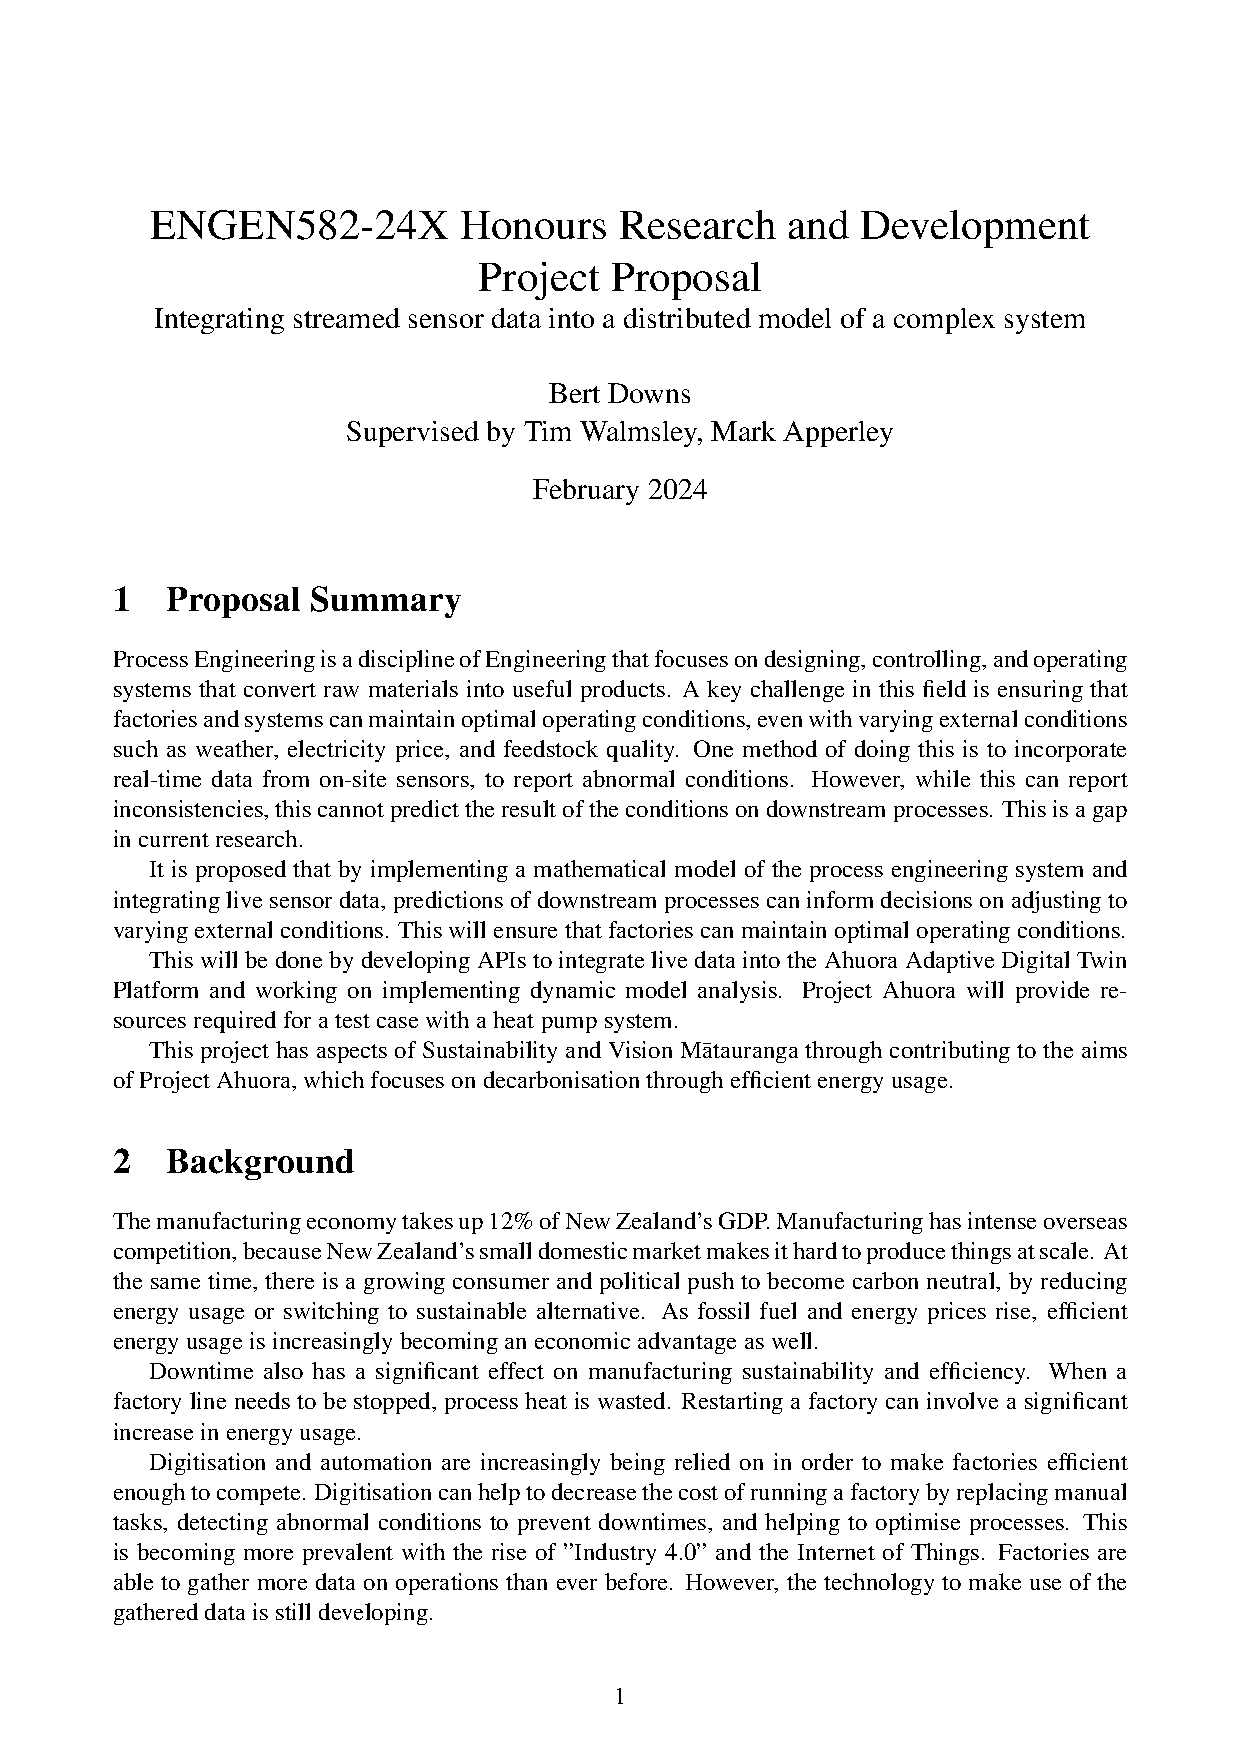
\includepdf[pages=1-4]{proposal.pdf}

% \begin{landscape}
%     \includepdf[pages=5,angle=90]{proposal.pdf}
% \end{landscape}

% \chapter{Literature Review} \label{sec:litreview}
% The literature review is included as an appendix on the following page.

% 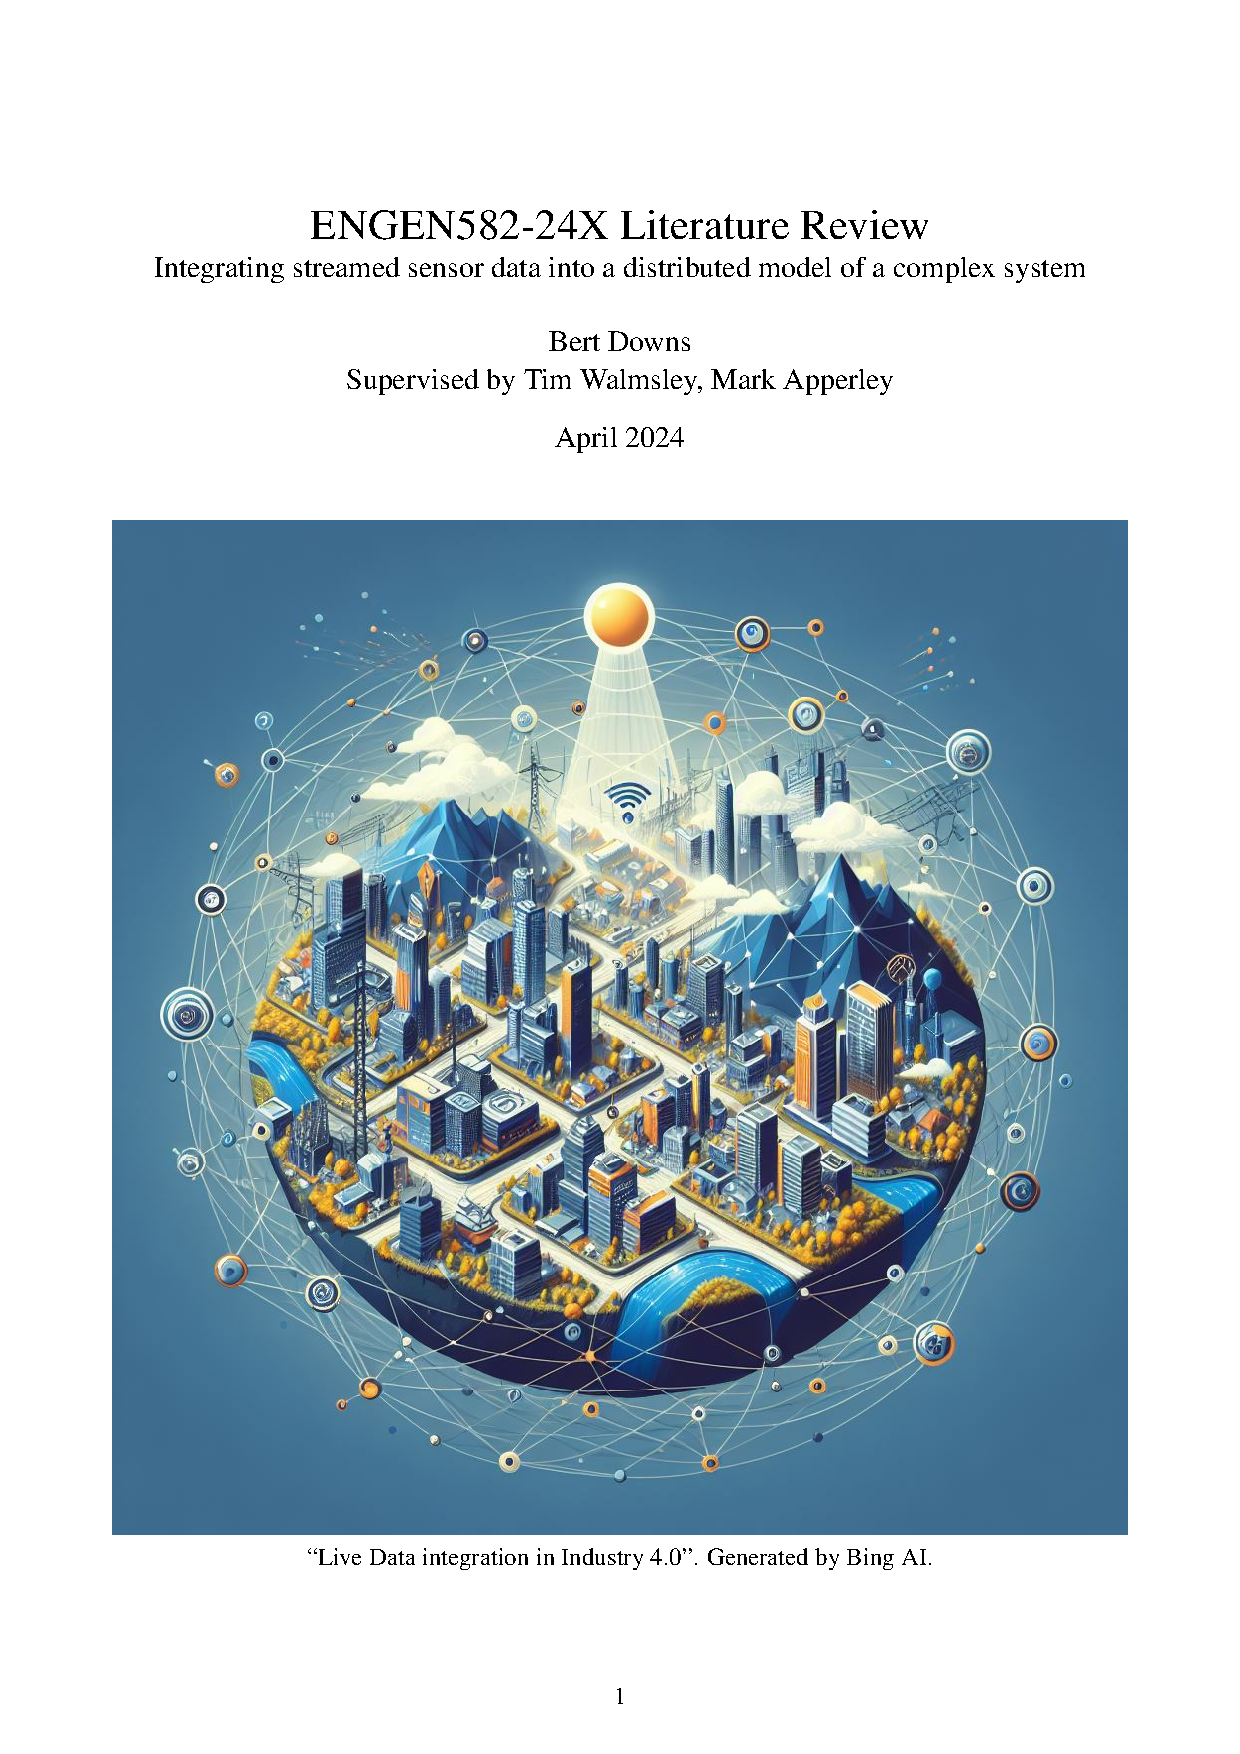
\includepdf[pages=-]{literature_review.pdf}

\end{appendices}
\end{document}